% !TEX root = ../../Main.tex
\section{Neural Networks}

Machine learning covers algorithms that find patterns in data and act on them, without being programmed with the rules in advance. Tom Mitchell states the idea as follows \cite{mitchell_machine_1997}:
\begin{quote}
"A computer program is said to learn from experience E with respect to some task T and some performance measure P, if its performance on T, as measured by P, improves with experience E."
\end{quote}
The definition is useful here because it describes exactly what a trading agent does. The task is choosing a position. The performance measure is the money that position makes. The experience is the market data the agent has already seen. Neural networks, the subject of this section, are the class of models used to represent that behaviour.

\subsection{Fundamentals and History}

Neural Networks (NN) are algorithms designed for pattern recognition. They are named after the human brain, because their structure is similar to it. In the brain, a neuron receives signals through structures called dendrites and processes them in the nucleus. It then passes the result down its axon to the dendrites of nearby neurons. A neural network works in a similar way. Each node is an artificial neuron. It receives an input, processes it with a mathematical function and passes the output to the next layer of nodes. In both cases, the strength and the type of the connections between neurons decide how the network behaves \cite{goodfellow_deep_2016}. \Cref{Figure:HumanNeuronVsArtificialNeuron} illustrates these ideas.

\begin{figure}[htb!]
\centering
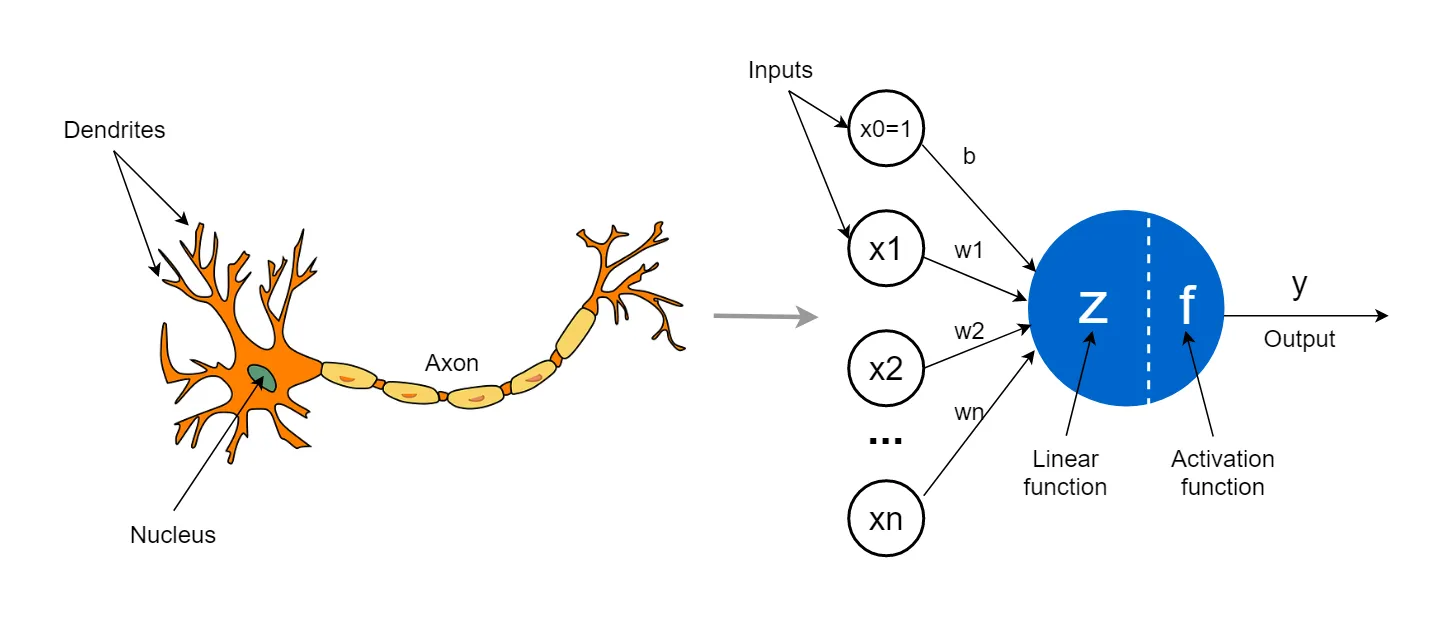
\includegraphics[width=0.7\textwidth]{Images/HumanNeuronVsArtificialNeuron.png}
\caption{Human Neuron compared to an Artificial Neuron \cite{pramoditha_human_nodate}.}
\label{Figure:HumanNeuronVsArtificialNeuron}
\end{figure}

The idea of neural networks goes back to the 1950s and the perceptron, a simple model of a biological neuron developed by Frank Rosenblatt \cite{rosenblatt_perceptron_1958}. The perceptron was the start of NN research. However, it could only learn linearly separable datasets, in which a straight line or a flat plane can separate the classes. This limit led to some periods of low interest in the field, known as ``AI winters''. A major advance came in the 1980s with the backpropagation algorithm. It allowed complex multilayer neural networks to learn patterns in datasets that are not linearly separable \cite{rumelhart_learning_1986}.

\subsection{Key Concepts and Feed-Forward}

In a neural network, the feed-forward computation in each layer \( l \) uses the output of the layer before it. For the first layer, this input \( x \) is the raw data itself. For the later layers, it is the output of the previous layer, \( h^{(l-1)}(x) \). The computation in each layer can be written as \cite{goodfellow_deep_2016}:

\begin{equation}
z^{(l)}(x) = W^{(l)} h^{(l-1)}(x) + b^{(l)}
\end{equation}

Here, the weight matrix \( W^{(l)} \in \mathbb{R}^{K_l \times K_{l-1}} \) and the bias vector \( b^{(l)} \in \mathbb{R}^{K_l} \) are used in the computation of layer \( l \). \( K_l \) is the number of neurons, or units, in layer \( l \), and \( K_{l-1} \) is the number of neurons in the previous layer \( l-1 \). For the first layer, \( W^{(1)} \in \mathbb{R}^{K_1 \times D} \), where \( D \) is the size of the input data. The activation function \( g \) is then applied to the pre-activation \( z^{(l)}(x) \in \mathbb{R}^{K_l} \) to give the activated output \( h^{(l)}(x) \in \mathbb{R}^{K_l} \) \cite{goodfellow_deep_2016}:

\begin{equation}
h^{(l)}(x) = g(z^{(l)}(x))
\end{equation}

The choice of activation function matters in two places. In the hidden layers, the function must be non-linear. A stack of linear layers is equal to a single linear transformation, so the network would gain nothing from its depth. In the output layer, the task decides the function. A bounded function is used when the output must stay within a range, and no activation is used when it does not \cite{goodfellow_deep_2016}. \Cref{Tables:ActivationFunctions} summarises the most common activation functions.

% !TEX root = ../Main.tex
\begin{table}[htb!]
\centering
\footnotesize
\caption{Summary of the most common Activation Functions \cite{goodfellow_deep_2016}.}
\label{Tables:ActivationFunctions}
\begin{tabularx}{\textwidth}{@{}lXl@{}}
\toprule
\textbf{Activation Function} & \textbf{Formula} & \textbf{Description} \\
\midrule
Linear & \( a(x) = x \) & Suitable for regression tasks. \\
\addlinespace
Sigmoid & \( \sigma(x) = \frac{1}{1 + e^{-x}} \) & Maps inputs to (0, 1), for binary classification. \\
\addlinespace
Hyperbolic Tangent & \( \tanh(x) = \frac{e^{x} - e^{-x}}{e^{x} + e^{-x}} \) & Maps inputs to (-1, 1), with stronger gradients than sigmoid. \\
\addlinespace
ReLU & \( \text{ReLU}(x) = \max(0, x) \) & Leads to sparse activation, helps gradient flow. \\
\addlinespace
Softmax & \( \text{Softmax}(z)_i = \frac{e^{z_i}}{\sum_{k=1}^K e^{z_k}} \) & Turns raw scores (logits) into probabilities, for multi-class classification. \\
\bottomrule
\end{tabularx}
\end{table}

\subsection{Learning using Backpropagation}

Neural networks learn by adjusting their weights and biases step by step, to reduce the error between the predicted outputs and the true target values. A loss function measures this error and guides the learning. The goal is to find the parameters that minimise the loss function. Different problems need different loss functions, such as mean squared error for regression tasks and cross-entropy for classification \cite{goodfellow_deep_2016}. \Cref{Tables:LossFunctions} gives their formulas.

% !TEX root = ../Main.tex
\begin{table}[htb!]
\centering
\footnotesize
\caption{Summary of the most common Loss Functions \cite{goodfellow_deep_2016}.}
\label{Tables:LossFunctions}
\begin{tabularx}{\textwidth}{@{}lXl@{}}
\toprule
\textbf{Loss Function} & \textbf{Formula} & \textbf{Application} \\
\midrule
Mean Squared Error (MSE) & \( \frac{1}{n} \sum_{i=1}^n (y_i - \hat{y}_i)^2 \) & Regression \\
\addlinespace
Negative Log-Likelihood (Cross-Entropy) & \( -\sum_{i=1}^n y_i \log(\hat{y}_i) \) & Classification \\
\bottomrule
\end{tabularx}
\end{table}

The main algorithm used to train neural networks is called backpropagation \cite{rumelhart_learning_1986}. It computes the gradient of the loss function with respect to the weights and biases of the network. The gradient points in the direction of steepest increase of the loss. \Cref{Codes:GradientLossFunction} shows how these gradients are calculated. Gradient descent then moves the weights and biases in the opposite direction, which reduces the loss. Its variants, listed with their formulas in \Cref{Tables:GradientDescent}, suit different data and computing needs. Batch gradient descent uses the whole dataset for each update. It is stable but expensive on large datasets. Stochastic gradient descent updates the parameters after every data point. It is faster but noisier. Mini-batch gradient descent updates on subsets of the data. It is the compromise used in practice \cite{goodfellow_deep_2016}.

% !TEX root = ../Main.tex
\begin{algorithm}[htb!]
\DontPrintSemicolon
\KwRequire{\( f \): network function, \( \theta \): network parameters, \( x \): input data, \( y \): true label, \( l \): number of layers, \( L \): loss function}
Compute the output of the network \( \hat{y} = f(x; \theta) \)\;
Compute the gradient of the loss function with respect to the output layer before activation:\;
\( \nabla_{z^{(l+1)}}L(f(x; \theta), y) = \frac{\partial L(f(x; \theta), y)}{\partial \hat{y}} \cdot \frac{\partial \hat{y}}{\partial z^{(l+1)}} \)\;
\For{\( \ell = l+1 \) to \( 1 \)}{
    Compute gradients of hidden layer parameters:\;
    \( \nabla_{W^{(\ell)}}L(f(x; \theta), y) = \nabla_{z^{(\ell)}}L(f(x; \theta), y) \cdot h^{(\ell-1)T} \)\;
    \( \nabla_{b^{(\ell)}}L(f(x; \theta), y) = \nabla_{z^{(\ell)}}L(f(x; \theta), y) \)\;
    Compute gradient of previous hidden layer:\;
    \( \nabla_{h^{(\ell-1)}}L(f(x; \theta), y) = W^{(\ell)T} \cdot \nabla_{z^{(\ell)}}L(f(x; \theta), y) \)\;
    Compute gradient of previous hidden layer (before activation):\;
    \( \nabla_{z^{(\ell-1)}}L(f(x; \theta), y) = \nabla_{h^{(\ell-1)}}L(f(x; \theta), y) \odot g'(z^{(\ell-1)}) \)\;
}
\caption{Gradient of the Loss Function \cite{goodfellow_deep_2016}.}
\label{Codes:GradientLossFunction}
\end{algorithm}

In \Cref{Tables:GradientDescent}, the learning rate \( \eta \) is a hyperparameter that controls the size of each update. A rate that is too large overshoots the minimum. A rate that is too small converges slowly and can get stuck in a local minimum. Some methods adapt \( \eta \) during training. They change the step size as the optimisation goes on, and this deals with both problems. Normalising or standardising the input data has the same aim, because features on very different scales produce gradients on very different scales \cite{goodfellow_deep_2016}.

% !TEX root = ../Main.tex
\begin{table}[htb!]
\centering
\footnotesize
\caption{Summary of the most common Gradient Descent variants \cite{goodfellow_deep_2016}.}
\label{Tables:GradientDescent}
\begin{tabularx}{\textwidth}{@{}lXl@{}}
\toprule
\textbf{Algorithm} & \textbf{Formula} & \textbf{Description} \\
\midrule
Batch Gradient Descent & \(\theta := \theta - \eta \cdot \nabla_{\theta} J(\theta; X, y)\) & Updates the parameters using all the data \\
\addlinespace
Mini-Batch Gradient Descent & \(\theta := \theta - \eta \cdot \nabla_{\theta} J(\theta; X^{(i:i+n)}, y^{(i:i+n)})\) & Updates the parameters using subsets of the data \\
\addlinespace
Stochastic Gradient Descent & \(\theta := \theta - \eta \cdot \nabla_{\theta} J(\theta; x^{(i)}, y^{(i)})\) & Updates the parameters after each data point \\
\bottomrule
\end{tabularx}
\end{table}

\subsection{Bias-Variance Trade-off and Model Generalisation}

How well a neural network generalises, that is, how well it works on data it has not seen, depends on a balance between bias and variance. Bias leads to underfitting. The model makes assumptions that are too simple and misses the real trends in the data. Variance leads to overfitting. The model is too complex and treats noise as if it were a signal. Both give poor results on new data. This matters in Forex trading, because the signal being sought is weak and the noise around it is large. Cross-validation is often used to measure how well a model generalises, on separate training, validation and testing datasets. Regularisation methods such as L1 and L2 limit the complexity of a model by adding penalties to the loss function. Dimensionality reduction methods such as principal component analysis reduce the number of inputs the model has to fit. Together, these methods make it more likely that the model performs well on out-of-sample data, which is data not used in training \cite{goodfellow_deep_2016}. This work divides the period into training, validation and testing windows, described in \Cref{Chapter:Implementation}. The performance on the validation window decides which model is kept. Complexity is not controlled through a penalty added to the loss.

\subsection{Architectures for Sequential Data}

The network described so far is feed-forward. The whole input is given at once, and the output depends only on that input. Financial data is a sequence, so an obvious question is whether a network that reads a sequence directly would do better.

Two families of networks do that. A recurrent neural network keeps an internal state that is carried from one step to the next, so each observation is read together with the ones before it. The long short-term memory network is the variant used in practice. It adds gates that control what the state keeps and what it drops. This stops the gradient from vanishing, that is, from shrinking towards zero, as it is propagated back over many steps \cite{goodfellow_deep_2016}. Attention-based networks reach the same goal in a different way. They let the network weigh every position in a window directly, instead of passing information along a chain.

Much of the work reviewed in \Cref{Chapter:RelatedWork} uses recurrent networks, and several of those studies report that they helped. This work does not use them, and this was a deliberate design decision. Recurrence is one way to give a network access to the past. Another way is to compute measures of the past explicitly and give them to the network as part of the input. The observation described in \Cref{Chapter:Implementation} uses the second way. It includes momentum and moving-average readings over horizons from one day to one year. The history that a recurrent state would have to learn to summarise is therefore measured directly and given to the network.

This choice has three consequences. First, a feed-forward network on engineered features has far fewer parameters than a recurrent network on raw prices. This matters when the signal is weak and the sample is one instrument over eleven years. Second, it is faster to train. Training speed decided how many independent runs were possible, and this turned out to matter more for the quality of the final result than any gain from a different architecture would have. Third, it keeps the input interpretable. Each feature is a named quantity with a known meaning, so when a policy behaves strangely, the observation can be inspected instead of guessed at.

This choice also has a cost. A recurrent network can, in principle, find a summary of the past that no fixed set of indicators contains. This work gives up that possibility. Whether it would have helped here has not been tested, and it is listed among the extensions in \Cref{Section:FutureWork}.

\subsection{Universal Approximation Theorem}

The universal approximation theorem, proved by Hornik, Stinchcombe and White in 1989, can be stated as follows \cite{hornik_multilayer_1989}:

\begin{quote}
A neural network with one hidden layer and a linear output can approximate any continuous function arbitrarily well, given enough hidden units.
\end{quote}

The theorem shows that neural networks are universal function approximators, and this is what justifies their use here. It means that a large enough network can represent the function that maps market observations to a trading decision. It does not say whether such a function can be found from data, or whether it exists in a form stable enough to be useful. Those questions are the subject of the reinforcement learning methods covered next.